\subsection*{What is Communication Complexity}

Communication Complexity studies how much information two (or more) parties must exchange in order to solve a problem when the input is split between them. The key idea is that computation is easy, but communication is expensive. Instead of asking ``How long does the algorithm take?'', we ask:  

\[
\textit{How many bits do the parties need to communicate?}
\]



\textbf{Basic setup.}  
There are two players, traditionally called \textbf{Alice} and \textbf{Bob}.  
\begin{itemize}
    \item Alice holds input $x$
    \item Bob holds input $y$
    \item Together, they want to compute a function $f(x,y)$
\end{itemize}
They are allowed to send messages (bits) back and forth. The goal is to minimize the total number of bits communicated.\\[12pt]

\begin{figure}[H]
\centering
\begin{tikzpicture}[
node/.style={draw, rectangle, rounded corners, minimum width=2.5cm, minimum height=1cm},
cloud/.style={draw, ellipse, minimum width=3cm, minimum height=1cm}
]

\node[node] (A) at (0,0) {Alice: $x$};
\node[node] (B) at (8,0) {Bob: Data $y$};
\node[cloud] (F) at (4,-2.5) {Compute $f(x,y)$};

\draw[->] (A) -- (F);
\draw[->] (B) -- (F);

\draw[<->, thick] (A) -- node[above]{Communication} (B);

\end{tikzpicture}
\caption{Distributed computation}
\end{figure}


\newpage
\subsubsection*{Example 1: The Equality Problem}

In the \textbf{Equality} problem, Alice and Bob each hold an $n$-bit string:
\[
x \in \{0,1\}^n, \quad y \in \{0,1\}^n
\]
They want to determine whether
\[
f_{\text{EQ}}(x,y) =
\begin{cases}
1 & \text{if } x = y,\\
0 & \text{otherwise}.
\end{cases}
\]

\begin{figure}[h]
\centering
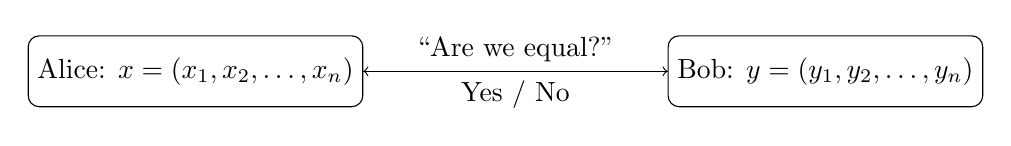
\begin{tikzpicture}[
node/.style={draw, rectangle, rounded corners, minimum width=2.2cm, minimum height=0.9cm}
]
\node[node] (A) at (0,0) {Alice: $x = (x_1, x_2, \ldots, x_n)$};
\node[node] (B) at (8,0) {Bob:  $y = (y_1, y_2, \ldots, y_n)$};

\draw[->] (A) -- node[above]{``Are we equal?''} (B);
\draw[<-] (A) -- node[below]{Yes / No} (B);
\end{tikzpicture}
\caption{Equality Example.}
\end{figure}

\subsubsection*{Why Equality Requires $n$ Bits}



\begin{figure}[H]
\centering
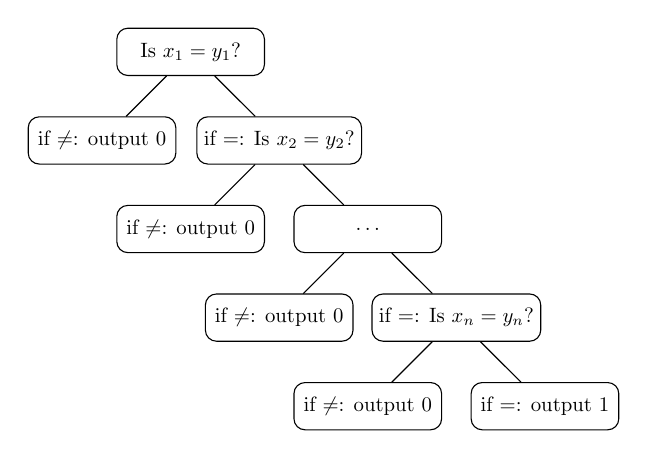
\begin{tikzpicture}[
  scale=0.75,                
  transform shape,          
  node/.style={draw, rounded corners, minimum width=2.5cm, minimum height=0.8cm},
  level distance=1.5cm,
  sibling distance=3cm
]

\node[node] {Is $x_1 = y_1$?}
  child { node[node] {if $\neq$: output $0$} }
  child { node[node] {if $=$: Is $x_2 = y_2$?}
    child { node[node] {if $\neq$: output $0$} }
    child { node[node] {$\dots$}
      child { node[node] {if $\neq$: output $0$} }
      child { node[node] {if $=$: Is $x_n = y_n$?}
        child { node[node] {if $\neq$: output $0$} }
        child { node[node] {if $=$: output $1$} }
      }
    }
  };
\end{tikzpicture}
\caption {Visual for Equality Proof}
\end{figure}


So from Figure 3, we can see how a deterministic protocol for Equality works.
The protocol checks the bits one by one. If at any position $i$ we find 
$x_i \neq y_i$, we can immediately output $0$. However, if the strings differ only in the last position, the protocol  has no way of knowing this until it checks that final bit. That means in the worst case, every single bit must be compared. Because of this, one party must effectively communicate all $n$ bits of their string to the other party in order to be completely certain whether $x = y$.\\

Thus, the deterministic communication complexity of Equality is $D(\text{EQ}) = n$


\newpage


\subsubsection*{Example 2: The Disjointness Problem}

In the \textbf{Disjointness} problem, Alice and Bob each have a subset of $\{1,2,\dots,n\}$, represented as binary vectors:
\[
x,y \in \{0,1\}^n,
\]
where $x_i = 1$ means Alice has element $i$, and similarly for Bob.

They want to determine whether their sets are disjoint:
\[
f_{\text{DISJ}}(x,y)=
\begin{cases}
1 & \text{if for all } i,\, x_i \cdot y_i = 0,\\
0 & \text{otherwise}.
\end{cases}
\]


\begin{figure}[h]
\centering
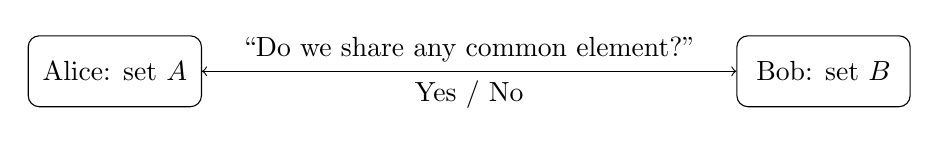
\begin{tikzpicture}[
node/.style={draw, rectangle, rounded corners, minimum width=2.2cm, minimum height=0.9cm}
]
\node[node] (A) at (0,0) {Alice: set $A$};
\node[node] (B) at (9,0) {Bob: set $B$};

\draw[->] (A) -- node[above]{``Do we share any common element?''} (B);
\draw[<-] (A) -- node[below]{Yes / No} (B);
\end{tikzpicture}
\caption{Disjointness: Alice and Bob must determine whether $A\cap B=\emptyset$.}
\end{figure}


\subsubsection*{Why Disjointness Requires $n$ Bits}

\begin{figure}[H]
\centering
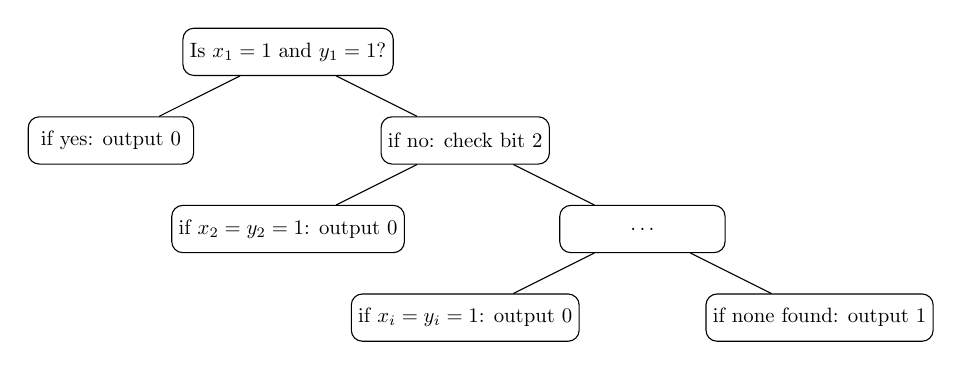
\begin{tikzpicture}[
  scale=0.75,
  transform shape,
  node/.style={draw, rounded corners, minimum width=2.8cm, minimum height=0.8cm},
  level distance=1.5cm,
  sibling distance=6cm
]

\node[node] {Is $x_1 = 1$ and $y_1 = 1$?}
  child { node[node] {if yes: output $0$} }
  child { node[node] {if no: check bit 2}
    child { node[node] {if $x_2=y_2=1$: output $0$} }
    child { node[node] {$\dots$}
      child { node[node] {if $x_i=y_i=1$: output $0$} }
      child { node[node] {if none found: output $1$} }
    }
  };
\end{tikzpicture}
\caption{Visual for Disjointness Proof}
\end{figure}

For Disjointness, Alice and Bob each have an $n$-bit string. We interpret $x_i = 1$ as Alice having element $i$ in her set, and similarly for Bob. The goal is to determine whether there exists an index $i$ such that $x_i = 1$ and $y_i = 1$. If such an index exists, the sets are not disjoint  and we output $0$. If no such index exists, we output $1$. From the figure, we see that the protocol must check every coordinate in the worst case. If the two sets intersect at some position, we can stop early. However, if they are disjoint except possibly at the very last position, the protocol cannot know this without checking all $n$ bits. This means that in the worst case, the parties must exchange information about every coordinate.\\

Thus, the deterministic communication complexity of Disjointness is $D(\text{DISJ}) = n$

